\section{Durchführung}
\label{sec:Durchführung}

\begin{figure}[H]
    \centering
        \centering
        
\includegraphics[width=0.8\textwidth]{Bilder/aufbau1.jpg}
        \caption{Aufbau der Apparatur (Eigenaufnahme).}
    \hfill
    \label{fig:7}
\end{figure}
\noindent In der obigen Abbildung befindet sich der vollständige Aufbau des Experiments.
In A ist die Drehschieberpumpe zu sehen. Diese ist von der Firma ILMVAC des Typs
300883/AKD16 und hat ein gelbes Ventil oberhalb (V1 genannt), sodass die Pumpe 
nach Belieben abgeriegelt werden kann. Die Drehschieberpumpe ist angeschlossen
an das TPG-202 von Pfeiffer Vacuum, einem kombinierten Piezo/Pirani-Sensor,
welcher für die Messungen mit der Drehschieberpumpe verwendet wird (Punkt C). 
Daneben befindlich ist die Turbopumpe in B mit einem schwarzen Ventil V3 sowie 
einem Sensor D1 in rot direkt darüber. Daran angebaut ist der Rezipient, eine
etwa $\qty{1.5}{\meter}$ lange Röhre aus Edelstahl. Letztlich ist daran noch
ein T-Stück angebaut, welches mit einem weiteren Sensor (D2) und Verschlussventilen
V4 (Belüftungsventil) und V5 (Dosierventil) versehen ist (siehe \autoref{fig:8})
\begin{figure}[H]
    \centering
        \centering
        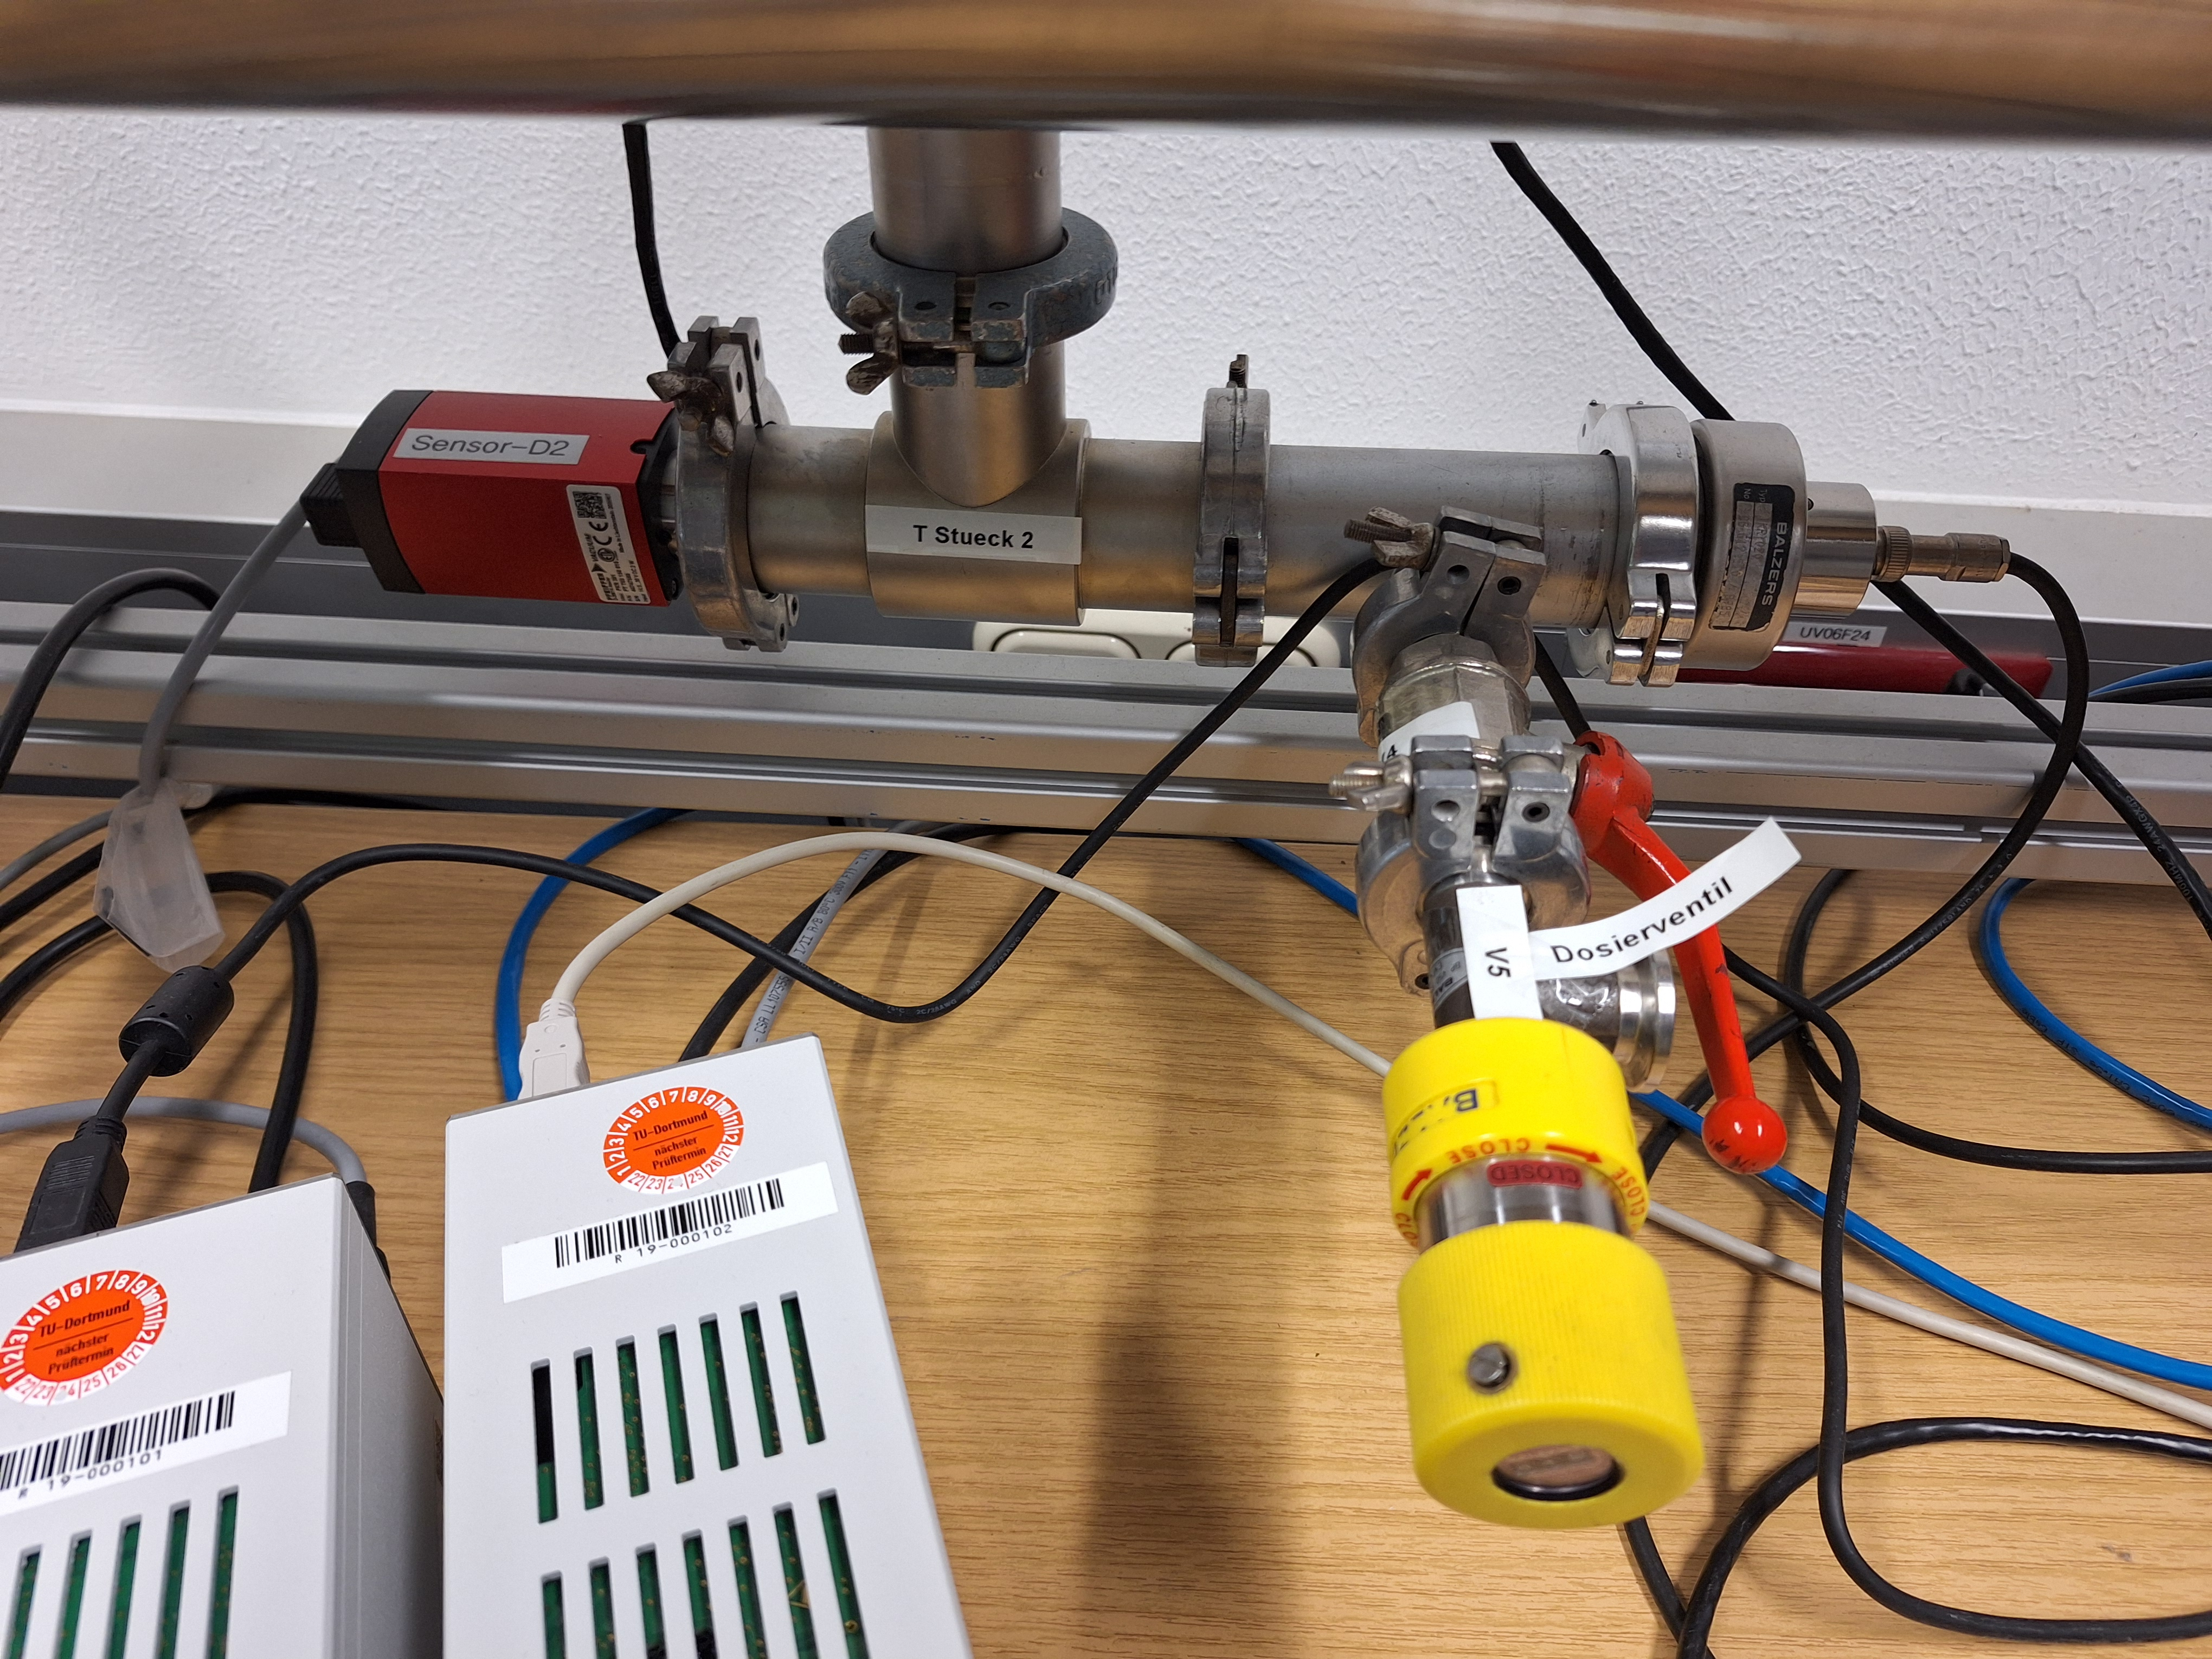
\includegraphics[width=0.7\textwidth]{Bilder/T.jpg}
        \caption{Nahaufnahme der Anbauten (Eigenaufnahme).}
    \hfill
    \label{fig:8}
\end{figure}
\noindent Die roten Sensoren D1 und D2 sind kombinierte PKR-360 von Pfeiffer
Vacuum, Pirani/Kaltkathoden Messgeräte. Diese sind verbunden mit den Ausgabegeräten
d1 und d2, dabei handelt es sich um TPG361, ebenfalls der Marke Pfeiffer Vacuum.
In E befindet sich ein Notebook, um die detektierten Drücke mithilfe der 
Thonny-Python-Programmierumgebung zu erfassen.

\subsubsection{TMP: Evakuierungskurve}
Nachdem durch Zusammenspiel von DP und TMP ein Druck von $\qty{5e-5}{\milli\bar}$
erreicht wurde, kann die Evakuierungskurve bestimmt werden. Es wird V3 geöffnet, 
sodass die TP mit dem Rezipienten verbunden ist. Gleichzeitig wird V5 so reguliert,
dass sich ein Druck von etwa $\qty{5e-5}{\milli\bar}$ einstellt. Es wird das 
Python-Skript gestartet und kurz darauf V4 und V5 geschlossen, sodass die Röhre evakuiert 
wird. Für 120 Sekunden wird nun der Druckabfall gemessen, dieser Vorgang für eine 
statistisch abgesicherte Mittelwertbildung fünfmal wiederholt. Am Ende stellt
sich ein Enddruck $p_E$ ein, dieser wird notiert.

\subsubsection{TMP: Leckratenmessung}
\label{sec:Leckratenmessung}
Bei geöffnetem Ventil V3 wird eine definierte Leckrate $p_g$ eingestellt. Dann 
wird  die TMP über V3 abgeriegelt und der Druckanstieg für 120 Sekunden gemessen.
Das wird gemacht für verschiedene Leckraten: $p_g = \qty{5e-5}{\milli\bar},
\qty{7e-5}{\milli\bar}, \qty{e-4}{\milli\bar}, \qty{2e-4}{\milli\bar}$.

\subsubsection{TMP: Einbau eines Testrohrs}
Im Folgenden wird ein Rohr von etwa zehn Zentimetern Länge eingebaut, ein Bild 
dessen befindet sich in \autoref{fig:9}.
\begin{figure}[H]
    \centering
        \centering
        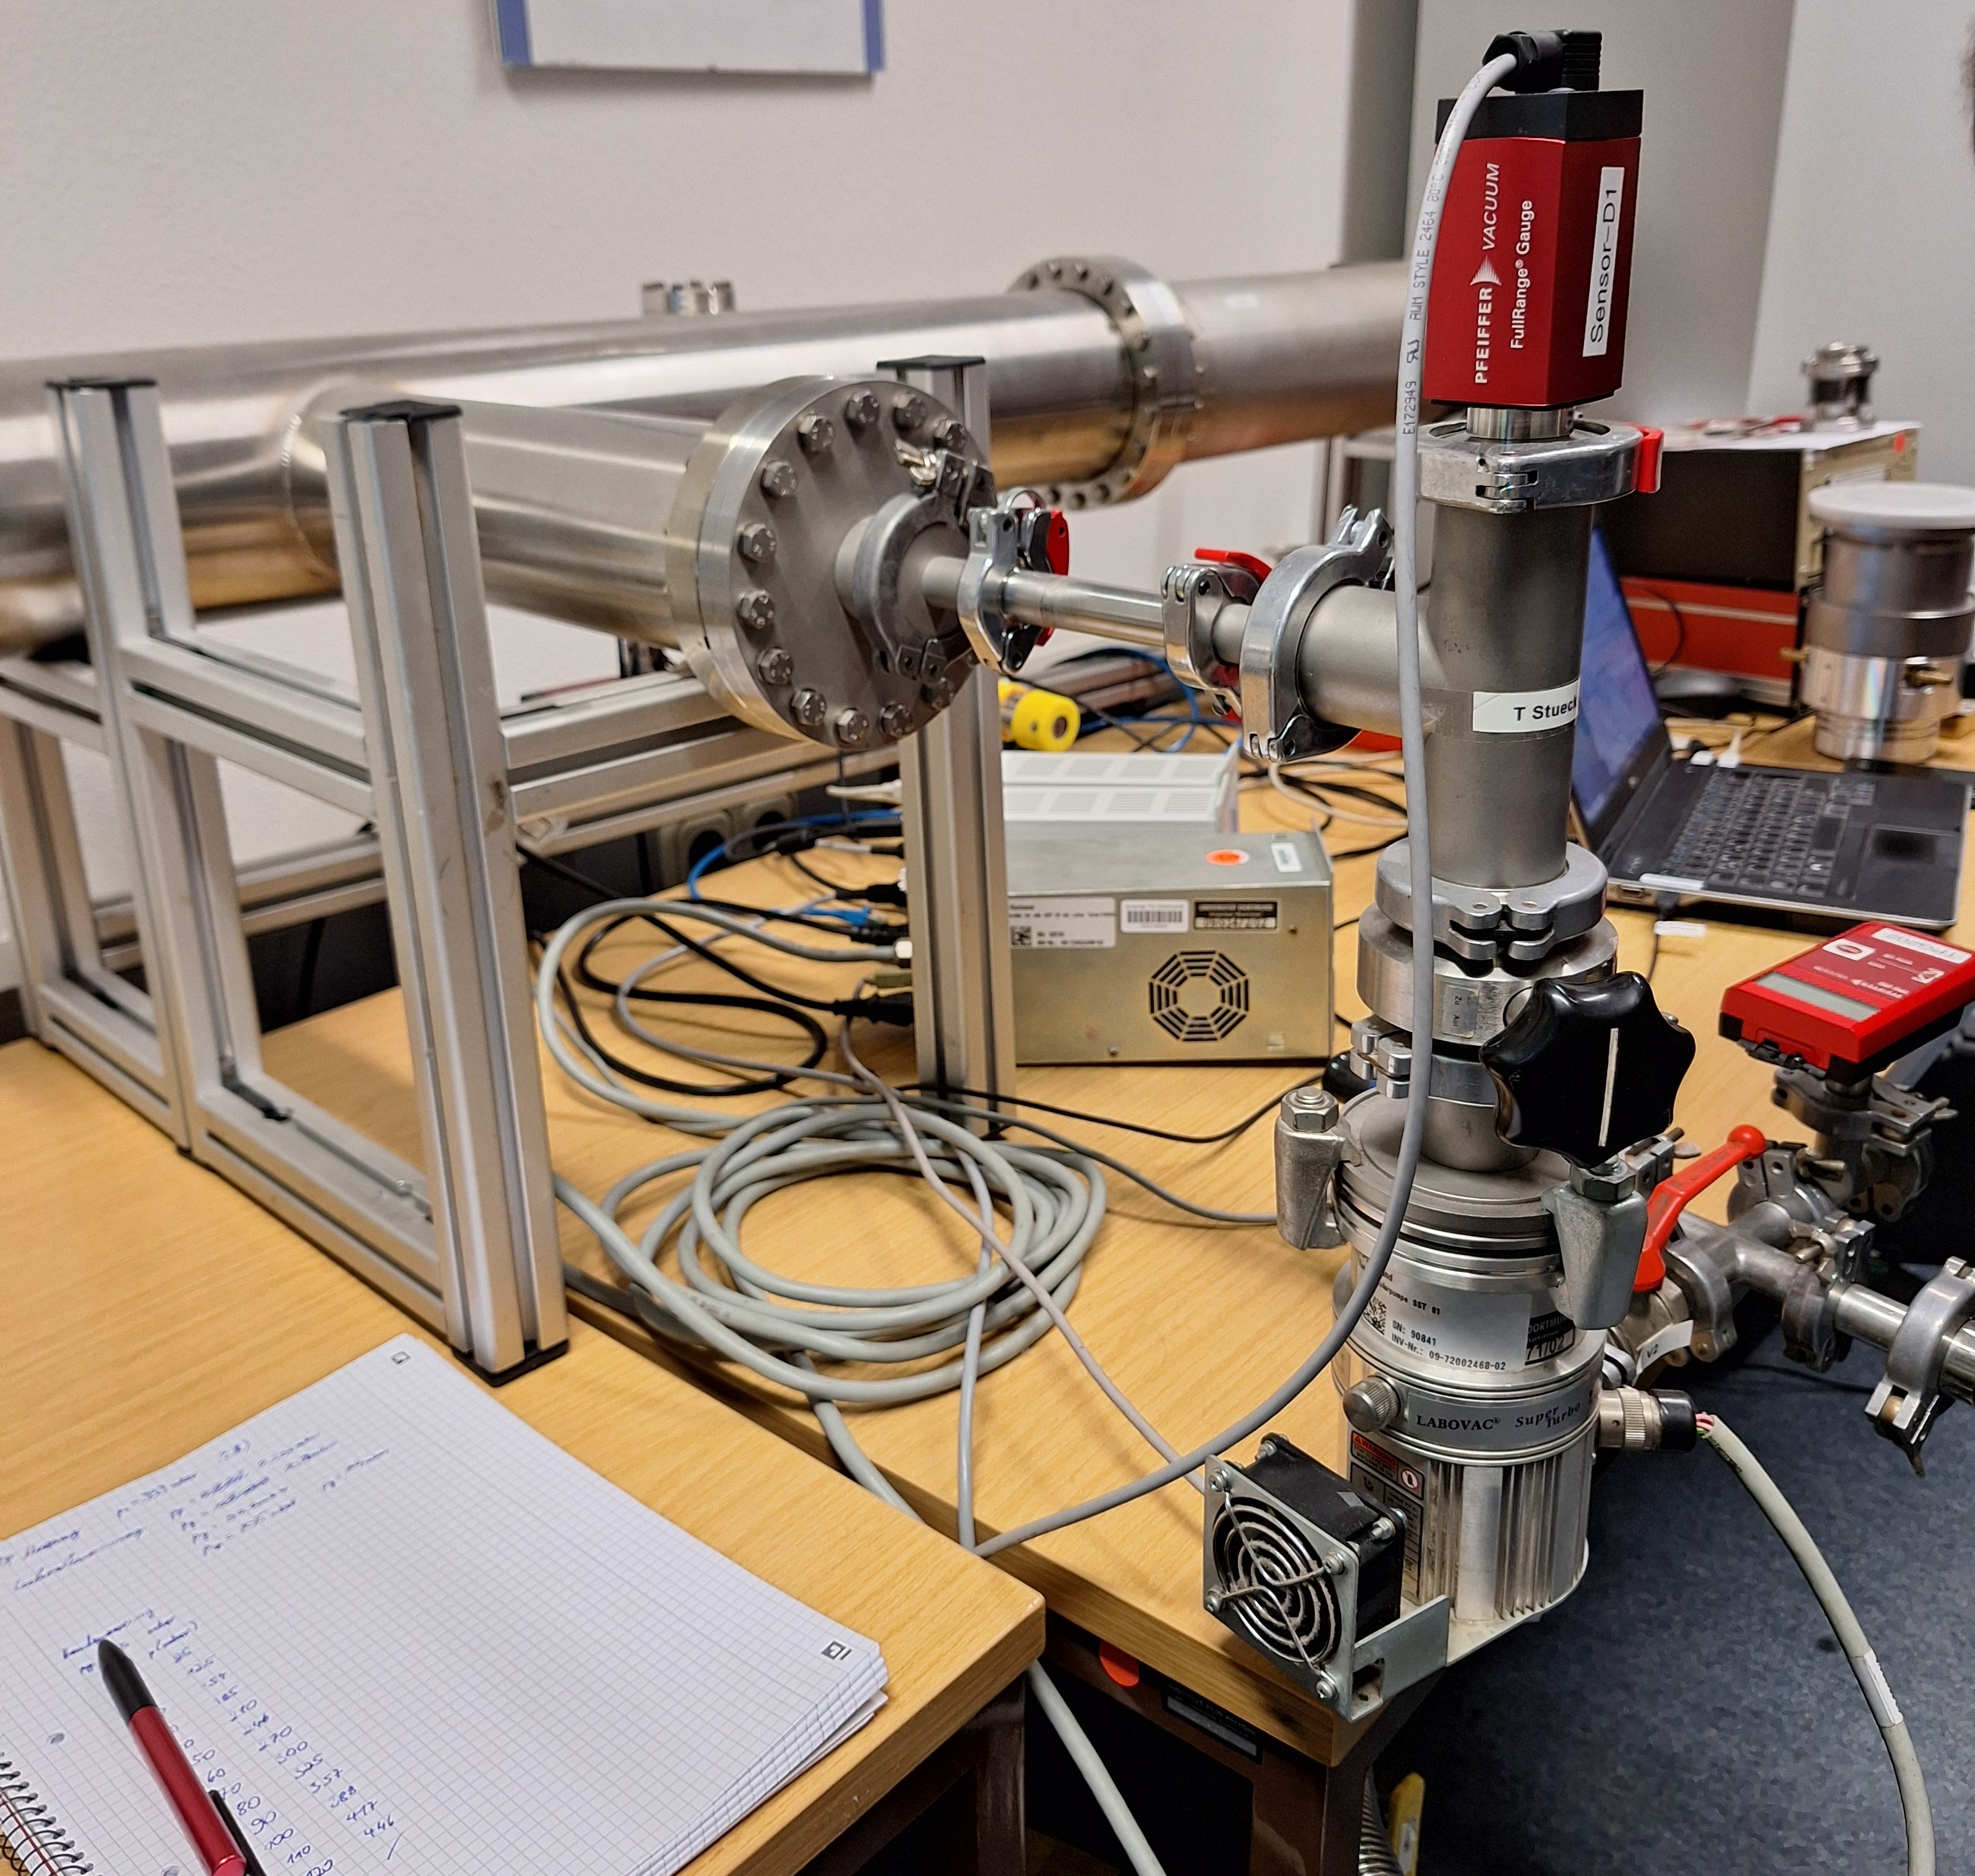
\includegraphics[width=0.7\textwidth]{Bilder/aufbau22.jpg}
        \caption{Eingebautes Testrohr zwischen TP und Rezipienten (Eigenaufnahme).}
    \hfill
    \label{fig:9}
\end{figure}
\noindent Durch die Verengung kommt es zu Strömungsverlusten, was darin resultiert,
dass die PKR-360 unterschiedliche Drücke ausgeben. Sobald sich ein Gleichgewichtsdruck 
einstellt, wird eine Leckratenmessung, wie in \autoref{sec:Leckratenmessung}, 
durchgeführt. Es wird der Druckunterschied der beiden Sensoren D1 und D2 
gemessen und durch Auswertung das effektive Saugvermögen vor und hinter der 
Engstelle bestimmt.

\subsubsection{DP: Aufbaukontrolle und Dichtigkeitsprüfung}
Zunächst wird der Aufbau gemäß \autoref{fig:7} überprüft. Die Drehschieberpumpe
wird eingeschaltet und das Absperrventil V1 geöffnet. Nach etwa 10 Minuten stellt
sich ein Enddruck von $p_E \approx \qty{0,03}{\milli\bar}$ am TPG-202 ein.
Damit gilt der Aufbau als ausreichend dicht.

\subsubsection{DP: Evakuierungskurve}
Der Rezipient wird über die Ventile V4 und V5 belüftet, bis der Normaldruck von
$\approx \qty{1000}{\milli\bar}$ erreicht ist. Dabei ist V1 geschlossen. 
Anschließend werden V4 und V5 geschlossen und das Python-Skript zur Datenerfassung
kann gestartet werden. Zum Zeitpunkt $t=0$ wird das Absperrventil V1 geöffnet.
Der Druckabfall wird einmal für 600 Sekunden mit dem TPG-202 aufgezeichnet.
Es stellt sich ein Druck $p_E$ ein, welcher notiert wird.

\subsubsection{DP: Leckratenmessung}
Bei laufender Pumpe und geöffnetem Absperrventil V1 sowie geöffnetem 
Belüftungsventil V4 wird über V5 ein konstanter Gleichgewichtsdruck $p_g$ im
Rezipienten eingestellt. Gemessen werden vier verschiedene Gleichgewichtsdrücke:
$p_g = \qty{0,5}{\milli\bar}, \qty{10}{\milli\bar}, \qty{50}{\milli\bar}$ und 
$\qty{100}{\milli\bar}$ (letzterer wird dreimal wiederholt, um eine Aussage über
den statistischen Fehler treffen zu können). Sobald der Druck konstant bleibt,
wird das Absperrventil V1 geschlossen, wodurch die Pumpe vom Rezipienten getrennt
wird. Gleichzeitig wird das Python-Skript zur Datenerfassung gestartet. Anschließend
wird der Druckanstieg im Rezipienten über eine Messdauer von 200 Sekunden mit
dem TPG-202 (Piezo-/Pirani-Kombisensor) aufgezeichnet. \cite{glossar}